\section{Vectors}

\subsection{Notation}

\blue{Complete reference page "vector and bases"}

\subsection{Cartesian coordinate system}
\blue{Complete in reference page "position and coordinates"}

\subsection{Polar coordinate system}
\blue{Complete in reference page "position and coordinates"}

\subsection{Units}
\blue{Complete in reference page "position and coordinates"}

\subsection{Unit vectors}
\blue{Complete in reference page "vector and bases"}

\subsection{Vectors bases}
\blue{Complete in reference page "vector and bases"}

\subsection{Changing bases}
\blue{Complete in reference page "vector and bases"}

\subsection{Projection and complementary projection}
\blue{Complete in reference page "vector and bases"}

\subsection{Change in length and direction}
\blue{Complete in reference page "Vector calculus"}

\subsection{Spherical Coordinates}
\blue{Complete in reference page "Spherical coordinates"}

\subsection{\red{Applications}}
    \subsubsection{\red{Spin lunch}}
    \red{This was mentioned in lecture but no actual example was given. It would be a good idea to include it.} Application for "Polar coordinates".

    \subsubsection{\red{Haystack antenna}}
    \red{This is mentioned in L09-Notes, slide 2. This topic needs to be formally expanded. Refer to Fig \ref{fig:AppAnetnna} }. Application for "Change of basis".
    \begin{figure}[h!]
        \centering
        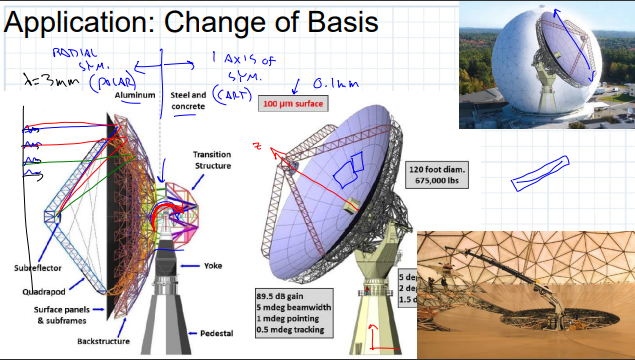
\includegraphics{VectorsFigs/AppAntenna.png}
        \caption{From L09-Notes, slide 2}
        \label{fig:AppAnetnna}
    \end{figure}
    
    \subsubsection{Shortest flight paths}
    \blue{Complete in reference page "Shortest flight paths"}. Application for Spherical coordinates.



